\documentclass{beamer}
\usepackage[english,russian]{babel}
\usepackage[utf8]{inputenc}
%\usepackage{smaller}
\usepackage{multicol}

%biblatex-gost
\usepackage[backend=biber, style=gost-authoryear, bibstyle=gost-authoryear, language=auto, babel=other, bibencoding=utf8, bibdoi=false, biburl=false,  movenames=false, sortcites = false]{biblatex}
\addbibresource{../txt/sophia_base.bib}


\mode<presentation>
%\mode<article>
% Стиль презентации
%\usetheme{Warsaw}
 \usetheme{Madrid}
%\usetheme{Marburg}
%\usetheme{Hannover}
%\usetheme{Singapore}
\usecolortheme{seahorse}



% в начале каждого раздела печатаем содержание с выделением текущего раздела
\AtBeginSection[]
{
  \begin{frame}<beamer>{Содержание}
    \tableofcontents[currentsection]
  \end{frame}
}




\begin{document}

\title[]{ОРГАНИЗАЦИЯ ПОСЕЛЕНИЙ {\it Macoma~balthica}~(Linnaeus,~1758) В ГРАДИЕНТАХ КЛЮЧЕВЫХ ПЕРЕМЕННЫХ СРЕДЫ ОСУШНОЙ ЗОНЫ БЕЛОГО И БАРЕНЦЕВА МОРЕЙ}
\author[С.А.~Назарова]{София Назарова \\ \medskip
	\footnotesize{Научный руководитель: д.б.н.~Н.~В.~Максимович}}
\institute[СПбГУ]{Санкт-Петербургский государственный университет}
\date{Санкт-Петербург, 2015} 

% Создание заглавной страницы
\frame{\titlepage} 





% Автоматическая генерация содержания
\frame{\frametitle{Содержание}\tableofcontents} 


%%%%%%%%%%%%%%%%%%%%%%%%%%%%%%%%%%%%%%%%%%%%%%%%%%%%%
		\section{Введение}
%%%%%%%%%%%%%%%%%%%%%%%%%%%%%%%%%%%%%%%%%%%%%%%%%%%%%
\begin{frame}{Вид {\it Macoma~balthica}}
	\begin{minipage}[b]{.39\linewidth}
		\begin{center}
%			\includegraphics[width=.9\textwidth]{Macoma_balthica.jpg}
		\end{center}
	\end{minipage}
	\begin{minipage}[b]{.49\linewidth}
{\it Macoma balthica} (L.,~1758)
		\begin{itemize}
			\item{Широко распространен}
			\item{Модельный объект популяционных исследований}
			\item{Легко доступен для изучения}
			\item{Важный элемент трофических цепей}
		%	\item{}
		\end{itemize}
	\end{minipage}
\end{frame}

\begin{frame}{Цели и задачи}
\begin{description}
	\item[Цель] Изучение гетерогенности поселений {\it Macoma balthica} в условиях арктических морей.

	\item[Задачи]  Изучение:
		\begin{enumerate}
    \item Изучение размерной структуры в различных местообитаниях %для описания эффектов внутрипопуляционной гетерогенности маком;
      \pause
    \item изучение многолетней динамики поселений маком;
      \pause
    \item изучение биотического и абиотического фона в поселениях;
      \pause
    \item изучение показателей линейного роста маком% для шкалирования изученных поселений по степени оптимальности условий обитания;
      \pause
    \item изучение численности спата %для изучения механизмов, определяющих пополнение локальных поселений.
		  \end{enumerate}
\end{description}
\end{frame}


%%%%%%%%%%%%%%%%%%%%%%%%%%%%%%%%%%%%%%%%%%%%%%%%%%%%%
		\section[География]{География исследований}
%%%%%%%%%%%%%%%%%%%%%%%%%%%%%%%%%%%%%%%%%%%%%%%%%%%%%
\begin{frame}{Белое море}
 \begin{center}
	\includegraphics[height=.8\textheight]{./White_sea.pdf}
 \end{center}
\end{frame}

\begin{frame}{Баренцево море}
 \begin{center}
	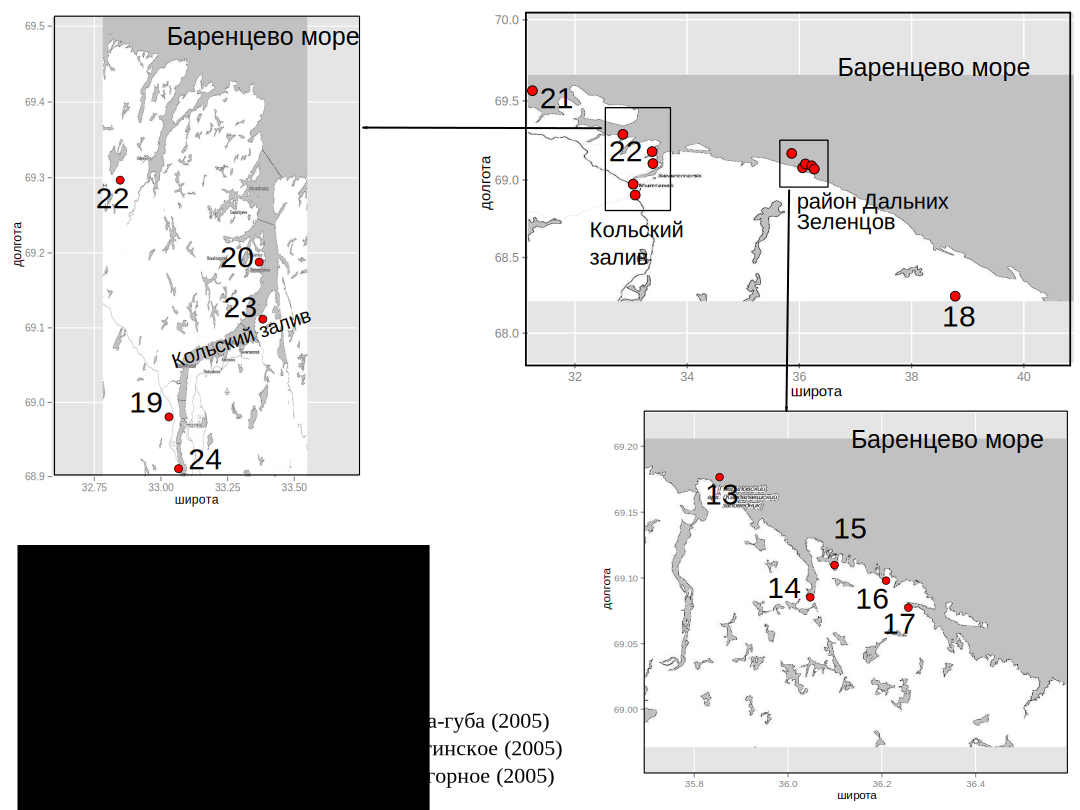
\includegraphics[height=.8\textheight]{./Barents_sea.pdf}
 \end{center}
\end{frame}

%%%%%%%%%%%%%%%%%%%%%%%%%%%%%%%%%%%%%%%%%%%%%%%%%%%%%
		\section[Обилие]{Обилие {\it Macoma balthica}}
%%%%%%%%%%%%%%%%%%%%%%%%%%%%%%%%%%%%%%%%%%%%%%%%%%%%%
\begin{frame}{Методы}
	\begin{itemize}
		\item Пробоотборник: Литоральные рамки площадью 1/30~м$^2$ / $3 \times$~1/30~=~1/10~м$^2$ (интегрированная проба) / зубчатый водолазный дночерпатель площадью~1/20~м$^2$
		\item Однократная съемка: от 3 до 36 проб
		\item Промывка: сито с диаметром ячеи $0,5 - 1$~мм 
		\item Численность: подсчет особей в пробах, пересчет в среднюю численность на м$^2$. 
		\item Биомасса: взвешивание с точностью до 10 мг / рассчет по формуле зависимости массы особи от ее длины (\cite{Maximovich_et_al_1993})
		\item Множественное сравнение средних с помощью теста Краскелла-Уоллеса
		\item Сравнительный материал: информация о средних численности и биомассе в европейской части ареала макомы (всего 39 источников о 52 поселениях)
	\end{itemize}
\end{frame}

\begin{frame}{Обилие {\it M.~balthica} в Белом море}
	\begin{minipage}[t]{.49\linewidth}
		\begin{center}
		{\footnotesize Численность}
			\includegraphics[width=\textwidth]{N2_area_White1.pdf}
		\end{center}
	\end{minipage}
%
	\begin{minipage}[t]{.49\linewidth}
		\begin{center}
		{\footnotesize Биомасса}
			\includegraphics[width=\textwidth]{B_Kanda_ru1.pdf}
		\end{center}
	\end{minipage}

{\tiny жирная горизонтальная линия~--- медианное значение показателя, 
границы <<ящика>>~--- 1 и 3 квартили, <<усы>>~--- 1,5 интерквартильного расстояния, 
точки - значения выпадающие за 1,5 интерквартильных расстояния. 
Числа в верхней части графика~--- среднее значение численности маком, экз./м$^2$.}

\end{frame}



\begin{frame}{Обилие {\it M.~balthica} в Баренцевом море}
	\begin{minipage}[t]{.49\linewidth}
		\begin{center}
		{\footnotesize Численность}
			\includegraphics[width=\textwidth]{N2_area_Barents1.pdf}
		\end{center}
	\end{minipage}
%
	\begin{minipage}[t]{.49\linewidth}
		\begin{center}
		{\footnotesize Биомасса}
			\includegraphics[width=\textwidth]{B_Barents_uchastki_ru1.pdf}
		\end{center}
	\end{minipage}

{\tiny жирная горизонтальная линия~--- медианное значение показателя, 
границы <<ящика>>~--- 1 и 3 квартили, <<усы>>~--- 1,5 интерквартильного расстояния, 
точки - значения выпадающие за 1,5 интерквартильных расстояния. 
Числа в верхней части графика~--- среднее значение численности маком, экз./м$^2$.}
\end{frame}



\begin{frame}{Обилие {\it M.~balthica} в европейской части ареала}
	\begin{minipage}[t]{.49\linewidth}
		\begin{center}
		{\footnotesize Численность}
			\includegraphics[width=\textwidth]{Nmean_ru1.pdf}
		\end{center}
	\end{minipage}
%
	\begin{minipage}[t]{.49\linewidth}
		\begin{center}
		{\footnotesize Биомасса}
			\includegraphics[width=\textwidth]{Bmean_ru1.pdf}
		\end{center}
	\end{minipage}

{\tiny Средние значения показателей пропорциональны площади круга на карте}
\end{frame}


\begin{frame}{Положения выносимые на защиту}
 1. \textit{Macoma balthica} на литорали Белого и Баренцева моря образуют разные по структуре поселения.

\smallskip
На литорали Кандалакшского залива Белого моря и в Баренцевом море (Западный Мурман и Кольский залив) вид  формирует плотные поселения, в которых численность особей значительно варьирует во времени и может достигать нескольких тысяч экз./м$^2$, но наиболее типичны поселения маком с плотностью в несколько сотен экз./м$^2$. 

\smallskip
При этом среднее обилие \textit{M.~balthica} в Кандалакшском заливе Белого моря и в Кольском заливе Баренцева моря наибольшее в пределах европейской части ареала вида.

\smallskip
На литорали Восточного Мурмана Баренцева моря \textit{M.~balthica} не формирует плотных поселений, и ее численность редко превышает 100~экз./м$^2$.
\end{frame}
%%%%%%%%%%%%%%%%%%%%%%%%%%%%%%%%%%%%%%%%%%%%%%%%%%%%%
		\section[Динамика обилия]{Динамика плотности поселений {\it Macoma balthica} в Белом море}
%%%%%%%%%%%%%%%%%%%%%%%%%%%%%%%%%%%%%%%%%%%%%%%%%%%%%
\begin{frame}{Методы}
	\begin{itemize}
		\item 6 поселений {\it M.~balthica} в вершине Кандалакшского залива (Лувеньгские шхеры и Северный архипелаг): длина рядов от 7 до 20 лет.
		\item Сравнительный материал: 4 поселения {\it M.~balthica} в губе Чупа (данные из \cite{Maximovich_et_al_1991, Gerasimova_Maximovich_2013, Varfolomeeva_Naumov_2013})
		\item Расстояния между поселениями от 1 до 100 километров
		\item Множественное сравнение средних с помощью теста Краскелла-Уоллеса и пост-хок анализ с помощью теста Тьюки
		\item Попарное сравнение динамики численности в поселениях с помощью корреляции Мантеля
	\end{itemize}
\end{frame}

\begin{frame}{Динамика численности {\it M.~balthica} в вершине Кандалакшского залива}
	\begin{minipage}[t]{.49\linewidth}
		\begin{center}
			\includegraphics[width=\textwidth]{N2_dynamic_Luvenga_all.pdf}
		\end{center}
	\end{minipage}
%
	\begin{minipage}[t]{.49\linewidth}
		\begin{center}
			\includegraphics[width=\textwidth]{N2_dynamic_North_all.pdf}
		\end{center}
	\end{minipage}
\end{frame}

\begin{frame}{Синхронность динамики плотности поселений {\it M.~balthica} в Кандалакшском заливе Белого моря}
		\begin{center}
			\includegraphics[width=\textwidth]{mantel1.pdf}
		\end{center}
\end{frame}

\begin{frame}{Моделирование влияния температуры на численность {\it M.~balthica} в Кандалакшском заливе Белого моря}
$$\ln(N_{t1}) = 1,96 + 0,60 \times \ln(N_{t}) - 0,09 \times T_{wt1}$$
{\footnotesize $F = 37,04$; $p < 0,0001$. $R^2 = 0,6$} \\
	\begin{minipage}[t]{.49\linewidth}
		\begin{center}
			\includegraphics[width=\textwidth]{./lodNt_vs_logNt1_1.pdf}
		\end{center}
	\end{minipage}
%
	\begin{minipage}[t]{.49\linewidth}
		\begin{center}
			\includegraphics[width=\textwidth]{./Twt1_vs_logNt1_1.pdf}
		\end{center}
	\end{minipage}
\end{frame}

\begin{frame}{Положения выносимые на защиту}
2. Характер динамики численности \textit{Macoma balthica} в Белом и Баренцевом морях определяется варьированием численности однолетних особей в поселениях, которое зависит от нерегулярности пополнения поселений молодью, обусловленной в первую очередь различным уровнем выживаемости на первом году жизни.

\smallskip
Беломорские поселения демонстрируют элементы синхронности процессов пополнения, что связано с влиянием температуры на выживаемость маком в первый год жизни  (численность однолетних особей после холодных зим с устойчивым ледоставом оказывается относительно выше) и спецификой условий в локальном местообитании. 
\end{frame}
%%%%%%%%%%%%%%%%%%%%%%%%%%%%%%%%%%%%%%%%%%%%%%%%%%%%%
		\section[Динамика размерной структуры]{Характер размерной структуры поселений {\it Macoma balthica}}
%%%%%%%%%%%%%%%%%%%%%%%%%%%%%%%%%%%%%%%%%%%%%%%%%%%%%
\begin{frame}{Методы}
	\begin{itemize}
		\item Пробоотборник: Литоральные рамки площадью 1/30~м$^2$ / $3 \times$~1/30~=~1/10~м$^2$ (интегрированная проба) / зубчатый водолазный дночерпатель площадью~1/20~м$^2$
		\item Однократная съемка: от 3 до 36 проб
		\item Промывка: сито с диаметром ячеи $0,5 - 1$~мм 
		\item Измерения длины раковины и построение размерно-частотных распределений с шагом 1~мм
		\item 
	\end{itemize}
\end{frame}

\begin{frame}{Динамика численности {\it M.~balthica} в вершине Кандалакшского залива}
	\begin{minipage}[t]{.49\linewidth}
		\begin{center}
			\includegraphics[width=\textwidth]{N2_dynamic_Luvenga_all.pdf}
		\end{center}
	\end{minipage}
%
	\begin{minipage}[t]{.49\linewidth}
		\begin{center}
			\includegraphics[width=\textwidth]{N2_dynamic_North_all.pdf}
		\end{center}
	\end{minipage}
\end{frame}



\begin{frame}{Положения выносимые на защиту}
3. Динамика размерной структуры поселений {\it Macoma balthica} в Белом и Баренцевом представлена двумя типами. 

\smallskip
Более распространенный вариант: чередование бимодального и мономодального характера распределения особей по размерам. 
При этом первый пик формируют молодые особи (обычно длиной до 5~мм), а в случае бимодальной добавляется второй модальный класс из взрослых особей (в Белом море длиной 9 -- 12~мм, в Баренцевом 10 -- 17~мм). 
В Баренцевом море часто новое пополнение происходит до ухода старшей генерации и наблюдается три модальных группы.

\smallskip
В некоторых условиях формируется более редкий тип динамики с ежегодным повторением мономодальной размерной структуры. 
\end{frame}


%%%%%%%%%%%%%%%%%%%%%%%%%%%%%%%%%%%%%%%%%%%%%%%%%%%%%
		\section[Линейный рост]{Линейный рост {\it Macoma balthica}}
%%%%%%%%%%%%%%%%%%%%%%%%%%%%%%%%%%%%%%%%%%%%%%%%%%%%%
\begin{frame}{Методы}
	\begin{itemize}
		\item Особи {\it M.~balthica} из 7 поселений в Баренцевом море
		\item Измерения длины раковины и меток зимней остановки роста
		\item Аппроксимация при помощи уравнения Берталанфи: $L_{t} = L_{max} \times (1 - e^{(-k(t - t_{0}))})$, где $L_{max}$, $k$, $t_{0}$~--- коэффициенты, а $L_{t}$~--- длина раковины моллюска в возрасте $t$.
		\item Сравнительный анализ кривых роста произведен с учетом разброса эмпирических данных относительно регрессионной модели (\cite{Maximovich_1989}, компьютерная реализация Т.\:С.~Ивановой). 
		\item  Сравнительный материал: информация о ростовых характеристиках {\it M.~balthica} в Европейской части ареала (всего 15 источников о 25 поселениях)
		\item Широтное сравнение скорости роста с помощью параметра $\omega = L_{max} \times k$
	\end{itemize}
\end{frame}

\begin{frame}{Линейный рост {\it M.~balthica} в Баренцевом море}
	\begin{minipage}[t]{.58\linewidth}
		\begin{center}
			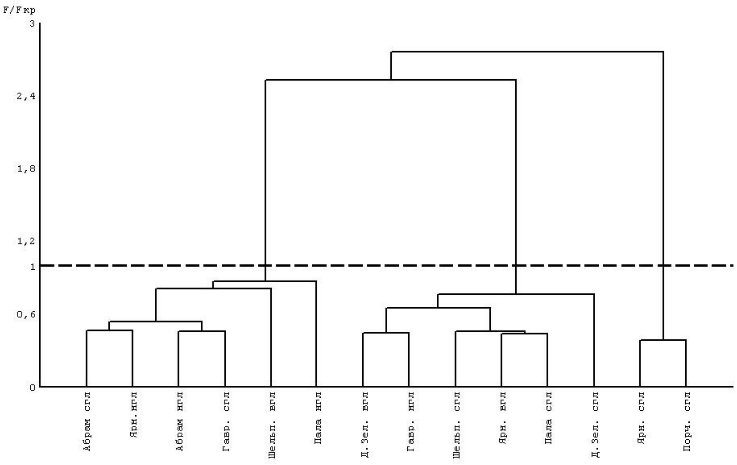
\includegraphics[width=\textwidth]{./dendrogramma_sravnenie_rosta_linear_all_gorizonts.pdf}
		\end{center}
	\end{minipage}
%
	\begin{minipage}[t]{.4\linewidth}
		\begin{center}
			\includegraphics[width=\textwidth]{./rost_clusters_all_crop.jpg}
		\end{center}
	\end{minipage}

1: \textcolor{violet}{Ярнышная СГЛ, Порчниха СГЛ}\\
2: \textcolor{cyan}{Пала СГЛ, Гаврилово СГЛ, Ярнышная СГЛ, Дальне-Зеленецкая СГЛ, Шельпино СГЛ}\\
3: \textcolor{orange}{Абрам-мыс, Пала НГЛ, Гаврилово СГЛ, Ярнышная НГЛ, Шельпино ВГЛ}
\end{frame}

\begin{frame}{\small Изменения среднего годового прироста особей {\it M.~balthica} в зависимости от начальной средней длины их раковин, мареографического уровня обитания (A) и условного смещения участка по побережью Мурмана на восток (Б)}
	\begin{minipage}[t]{.49\linewidth}
				{\small А}
			\begin{center}
				\includegraphics[width=\textwidth]{./prirost_otklik_mareography.jpg}
			\end{center}
		\end{minipage}
	\hfil %Это пружинка отодвигающая рисунки друг от друга
		\begin{minipage}[t]{.49\linewidth}
				{\small Б}
			\begin{center}
				\includegraphics[width=\textwidth]{./prirost_otklik_geography.jpg}
			\end{center}
		\end{minipage}
\tiny{1~--- Абрам-мыс, 2~--- Пала-губа, 3~--- Гаврилово, 4~--- Ярнышная, 5~--- Дальнезеленецкая, 6~--- Шельпино, 7~--- Порчниха.
Горизонты литорали: ВГЛ~--- верхний, СГЛ~--- средний, НГЛ~--- нижний}
\end{frame}


\begin{frame}{Линейный рост {\it M.~balthica} в Европейской части ареала}
	\begin{minipage}[t]{.52\linewidth}
		\begin{center}
			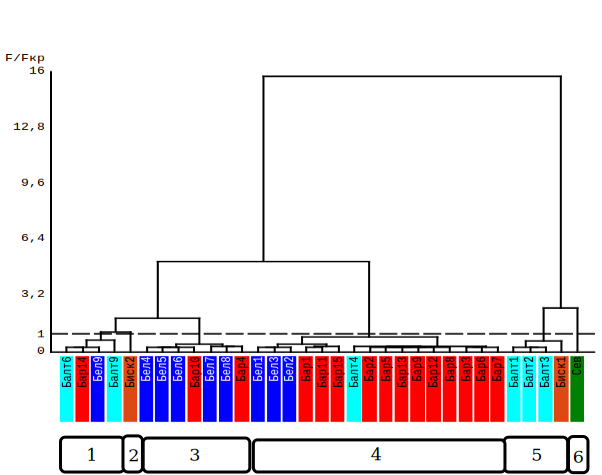
\includegraphics[width=\textwidth]{./Europe_clusters_usrednenie.pdf}
		\end{center}

Цветовые обозначения: \textcolor{red}{Баренцево море}, 
\textcolor{blue}{Белое море}, 
\textcolor{cyan}{Балтийское море}, 
\textcolor{green}{Северное море}, 
\textcolor{brown}{Бискайский залив}.
	\end{minipage}
%
	\begin{minipage}[t]{.45\linewidth}
		\begin{center}
			\includegraphics[width=\textwidth]{./Europe_growth_groups1.pdf}
		\end{center}
	\end{minipage}
\end{frame}

\begin{frame}{Широтные изменения скорости роста {\it M.~balthica} в Европейской части ареала}
		\begin{center}
			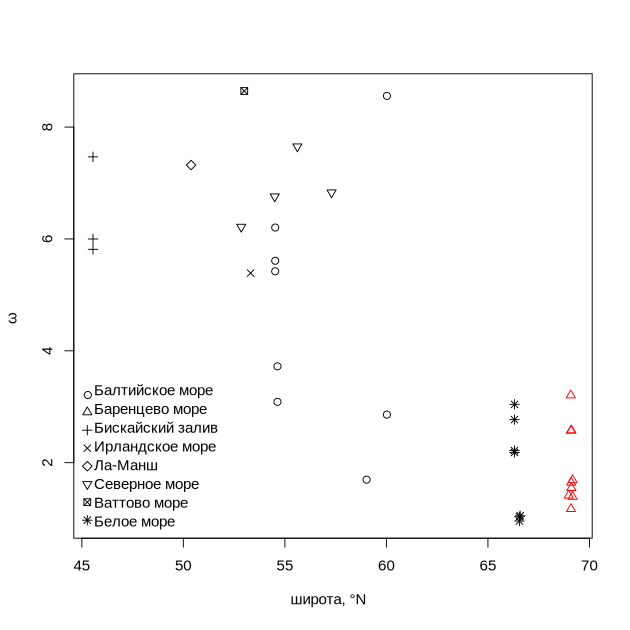
\includegraphics[height=.7\textheight]{./long_vs_omega_ru.pdf}
		\end{center}
корреляция Спирмена: $r_{s} = -0,60$, $p < 0,0001$

\end{frame}

\begin{frame}{Положения выносимые на защиту}
4. Особи {\it Macoma balthica} в Белом и Баренцевом морях отличаются наименьшей скоростью роста в пределах европейской части ареала вида. 
При этом внутригрупповая вариация роста особей \textit{M.~balthica} в поселениях Белого и Баренцева моря практически полностью перекрывается.
\end{frame}

%%%%%%%%%%%%%%%%%%%%%%%%%%%%%%%%%%%%%%%%%%%%%%%%%%%%%
		\section{Выводы}
%%%%%%%%%%%%%%%%%%%%%%%%%%%%%%%%%%%%%%%%%%%%%%%%%%%%%
\begin{small}

\begin{frame}{Выводы}
\addtocounter{enumi}{0}
	\begin{enumerate}
		\item Для Белого моря типичны поселения {\it Macoma balthica} с численностью в сотни экз./м$^2$ (при варьировании от единичных особей до более $8$~тыс.~экз./м$^2$). Варьирование обилия связано в первую очередь с численностью годовалых особей.
		      \pause
		\item Для литорали восточной части Мурманского побережья Баренцева моря типичны поселения {\it Macoma balthica} с численностью  менее 100~экз./м$^2$, и эти поселения не достигают плотностей, которые показаны для поселений на литорали Западного Мурмана и в Кольском заливе.
		      \pause
		\item Среднее обилие {\it Macoma balthica} в поселениях Белого моря и Кольского залива Баренцева моря выше, чем в других частях ареала, а биомасса сравнима со значениями в центральной части ареала. 
	\end{enumerate}
\end{frame}


\begin{frame}{Выводы}
	\begin{enumerate}
\addtocounter{enumi}{3}
		\item Макомы в Баренцевом море гетерогенны по скорости роста: Максимальный годовой прирост отмечен у особей среднего размера (возраста)~--- $6 - 9$~мм в среднем горизонте литорали. В пределах Восточного Мурмана средний годовой прирост особей {\it Macoma balthica} увеличивается в более восточных районах по сравнению с западными.
		      \pause
		\item В пределах европейской части ареала особи {\it Macoma balthica} из поселений в Белом и Баренцевом морях характеризуются минимальными скоростями роста. При этом нет принципиальных различий в скорости роста беломорских и баренцевоморских маком.
		      \pause
		\item Численность спата {\it Macoma balthica} в Белом море может варьировать на порядок в пределах незначительной акватории (от тысяч до десятков тысяч экз./м$^2$).
		      \pause
		\item Динамика численности годовалых особей {\it Macoma balthica} позволяет говорить о не ежегодном успехе пополнения их поселений в Белом море.
	\end{enumerate}
\end{frame}

\begin{frame}{Выводы}
	\begin{enumerate}
\addtocounter{enumi}{7}
		\item Динамика численности {\it Macoma balthica} в Кандалакшском заливе Белого моря демонстрирует элементы синхронности в поселениях, расположенных на расстоянии от 1 до 100~км. Кроме того, показано что численность маком оказывается выше в годы с холодными зимами.
		      \pause
		\item Динамика размерной структуры поселений {\it Macoma balthica} в Белом и Баренцевом представлена двумя типами. \\
Более распространенный вариант: чередование бимодального и мономодального распределение особей по размерам. При этом первый пик формируют молодые особи (обычно длиной до 5~мм), а в случае бимодальной добавляется второй модальный класс из взрослых особей (в Белом море длиной 9 -- 12~мм, в Баренцевом 10 -- 17~мм). В Баренцевом море часто новое пополнение происходит до ухода старшей генерации и наблюдается три модальных группы. 
В некоторых условиях формируется более редкий тип динамики с ежегодным повторением мономодальной размерной структуры.
	\end{enumerate}
\end{frame}

\end{small}

\appendix
		\section*{Формальные моменты}
\begin{frame}{Публикации по теме диссертации}
%	\nocite{*}
	%\printbibliography[heading=bibintoc]
%	\printbibliography[env=gostbibliography,sorting=ydnt]
\begin{itemize}
	\item{статьи: 5, из них 2 в журналах из списка ВАК}
	\item{тезисы докладов и материалы конференций: 9}
\end{itemize}
\end{frame}


\begin{frame}{Апробация работы}
\begin{itemize}
	\item{European Marine Biology Symposium: 2011, 2014, 2015}
	\item{Конференция ББС МГУ: 2004, 2008}
	\item{VI всероссийская школы по морской биологии <<Биоразнообразие сообществ морских и пресноводных экосистем России>>: 2007}
	\item{Научная сессия МБС СПбГУ: 2004, 2008, 2009, 2010}
	\item{Дерюгинские чтения: 2008}
	\item{Семинар кафедры ихтиологии и гидробиологии СПбГУ: 2003 -- 2015}
\end{itemize}
\end{frame}

		\section*{Благодарности}
\begin{small}
\begin{frame}{Благодарности}
\begin{multicols}{2}
	\begin{itemize}
		\item{Н.\:В.~Максимовичу}
		\item{В.\:М.~Хайтову}
		\item{Е.\:А.~Генельт-Яновскому}
		\item{Д.\:А.~Аристову} 
		\item{Ю.\:Ю.~Тамберг}
		\item{П.\:П.~Стрелкову}
		\item{А.\:В.~Полоскину}
		\item{К.\:В.~Шунькиной}
		\item{А.\:В.~Герасимовой}
		\item{А.\:Д.~Наумову}
		\item{И.\:А.~Коршуновой}
		\item{М.В.~Иванову}
		\item{М.\:В.~Макарову}
		\item{С.\:В.~и С.\:С.~Малавендам}
		\item{О.\:С.~Тюкиной}
		\item{И.\:П.~Прокопчук}
		\item{\fbox{Е.\:А. Нинбургу}}
		\item{\fbox{А.\:С.~Корякину}}
		\item{участникам Беломорской экспедиции ГИПС ЛЭМБ}
		\item{участникам студенческой Баренцевоморской экспедиции СПбГУ}
%		\item{участникам Беломорской экспедиции кафедры ихтиологи и гидробиологии СПбГУ}
		\item{администрации Кандалакшского заповедника}
	\end{itemize}
\end{multicols}
\end{frame}
\end{small}


\end{document}

